\section{Circuit Boards}
\label{sec:circuit_board}
After manufacture Tiny Tapeout chips are mounted onto small carrier boards with \qty{0.1}~inch pin headers. These carriers allow people with limited surface mount technology (SMT) assembly experience to build their own demonstration boards around the chips.

The carrier fits onto the demonstration board shown in Fig.~\ref{fig:demonstration_board}. The demonstration board is designed primarily for ease of use by beginners, though offers enough flexibility for power users. As all signals are below \qty{50}{\MHz} no special layout was needed in the design of the demonstration board.

The demonstration board provides:
\begin{itemize}
\item USB Type-C as a power connection,
\item \qty{1.8}{\V} and \qty{3.3}{\V} power supplies for core and IO,
\item \qty{20}{\MHz} oscillator,
\item Buttons for reset and single step clock,
\item An eight way DIP switch for inputs,
\item A nine way DIP switch for design selection,
\item A seven segment LED display for the outputs,
\item Headers for all IO, including two Digilent standard ports (PMOD),
\item A header to select the internal clock or to provide one externally,
\item A header to select an internal or external scan chain driver,
\item A header to engage an automatic clock divider in input pin zero.
\end{itemize}

\begin{figure}[!t]
\centering
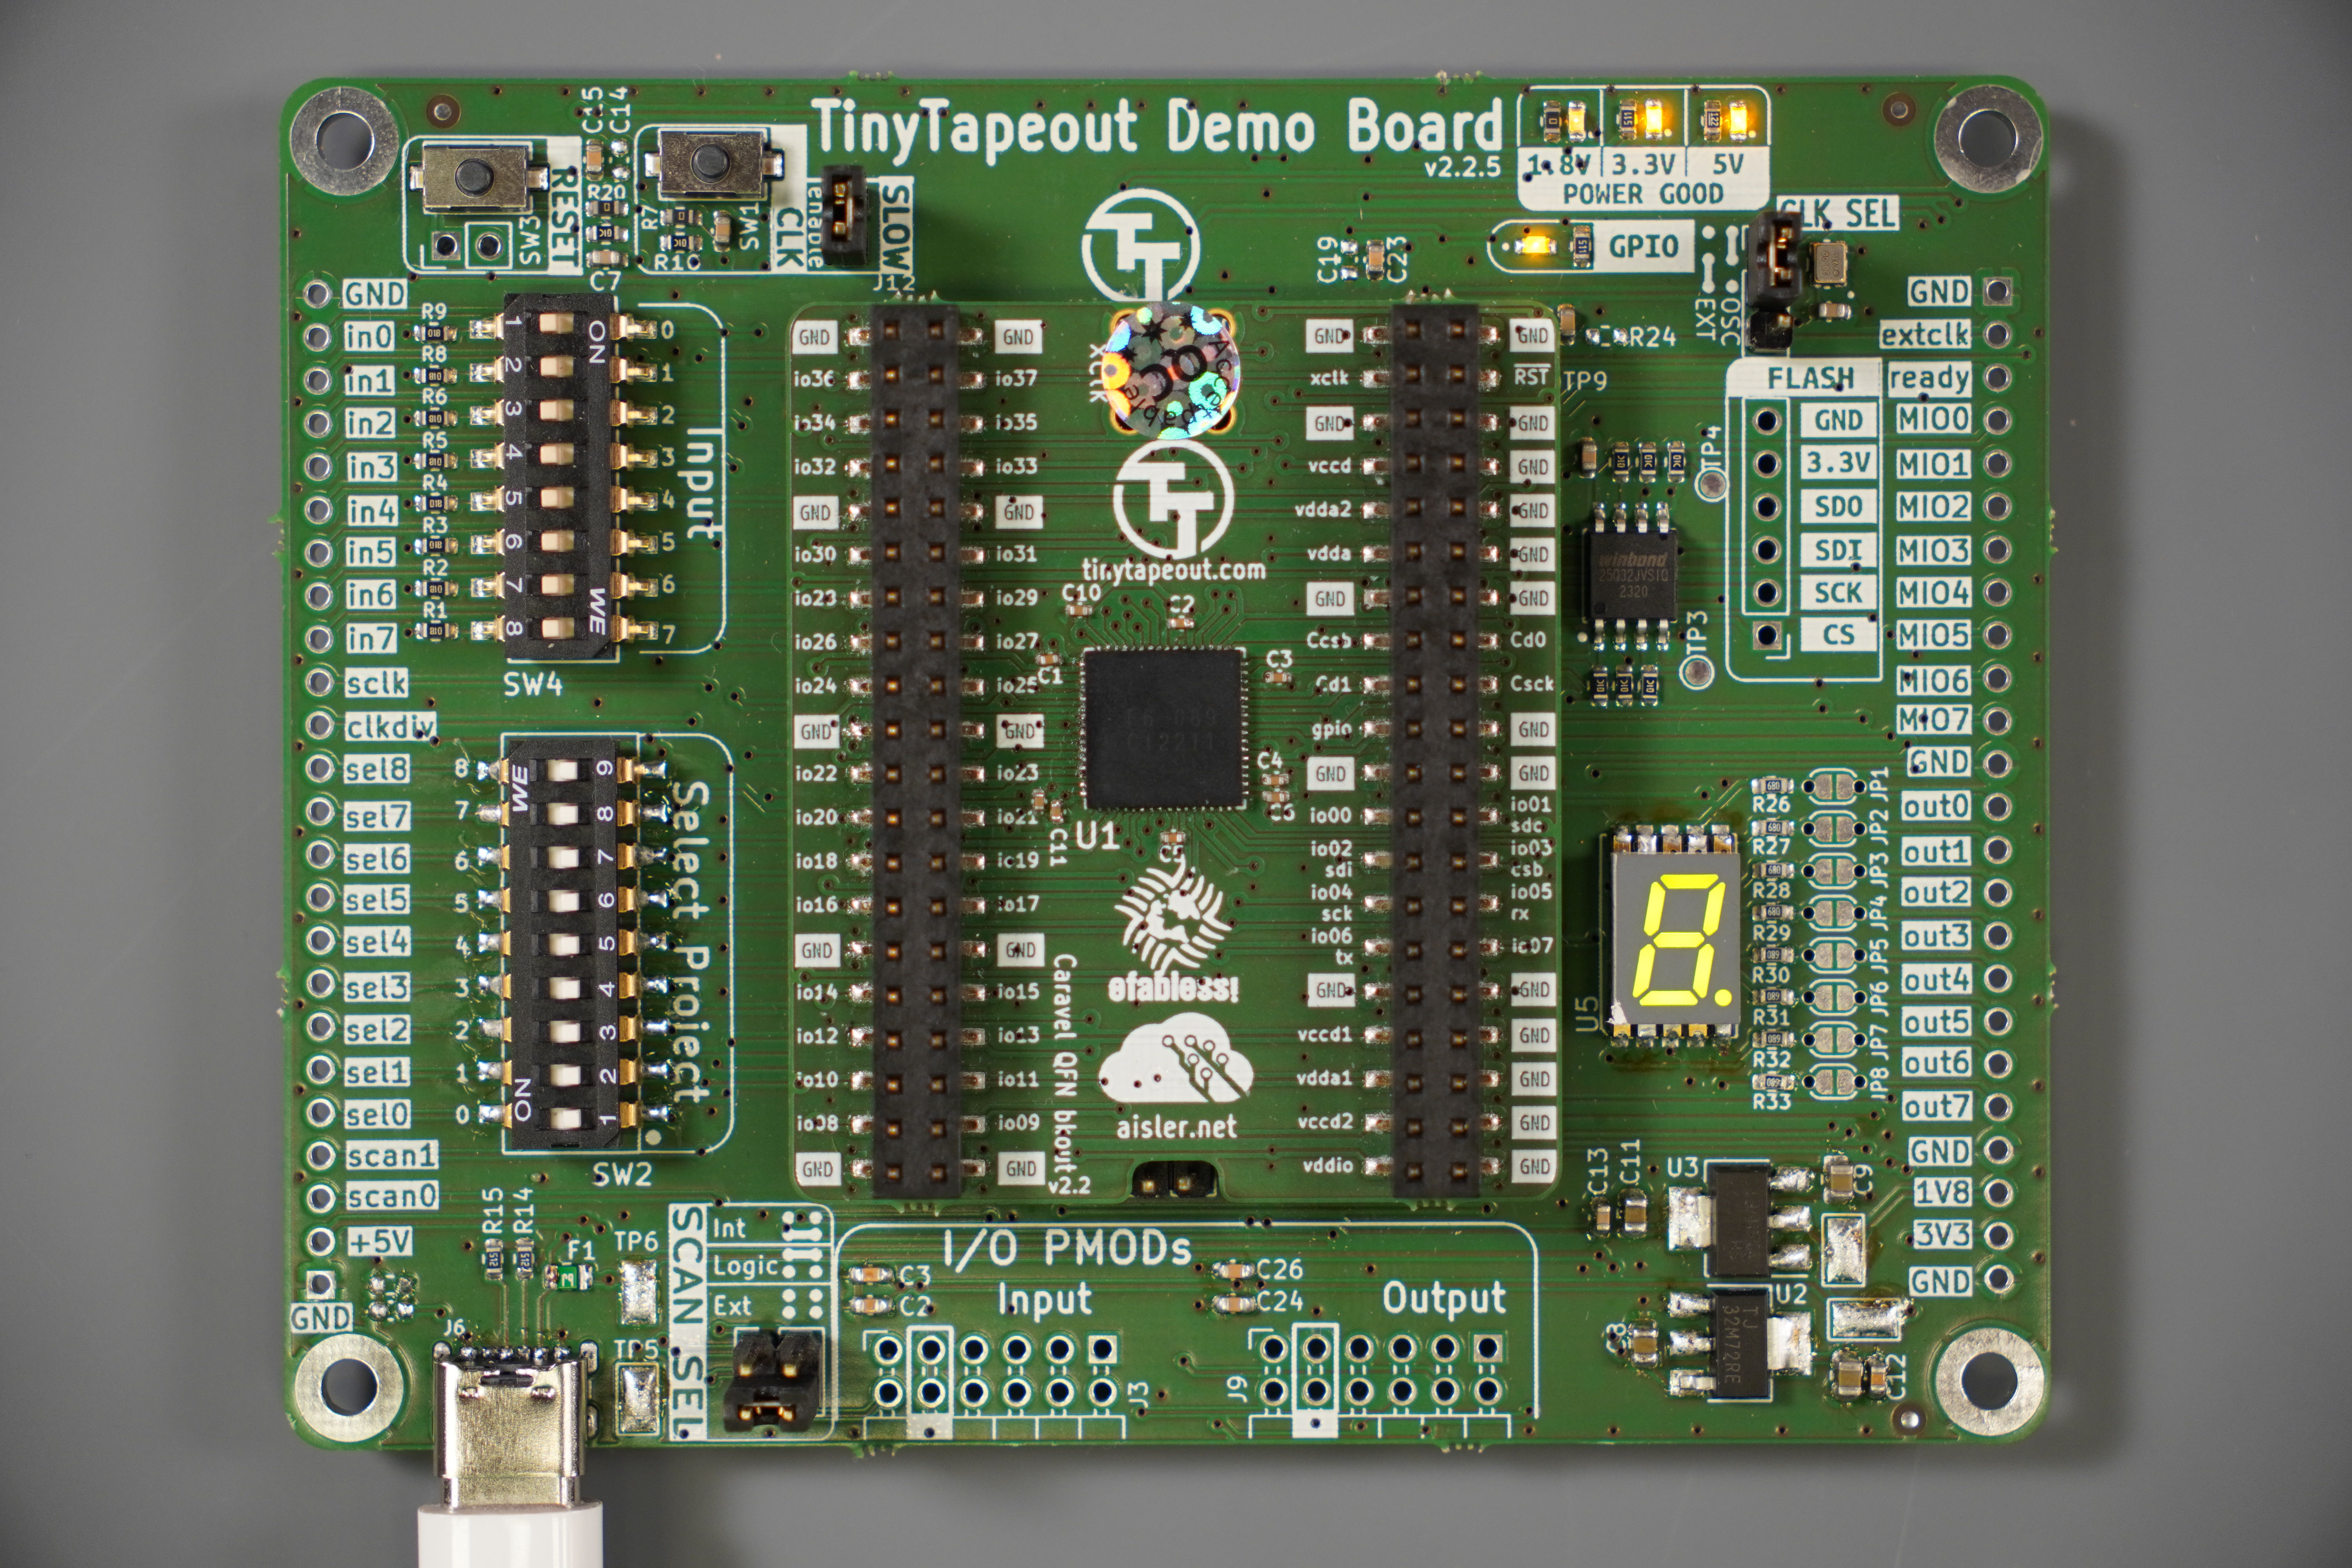
\includegraphics[width=0.5\textwidth]{./Figs/tt02 pcb assembled.JPG}
\caption{The demonstration board, which has been recorded as Certified Open Source Hardware ES000040~\cite{oshwacertification}.}
\label{fig:demonstration_board}
\end{figure}

The move away from the scan chain architecture in Tiny Tapeout 3.5 and Tiny Tapeout 4 necessitated the design of a new demonstration board (Fig.~\ref{fig:TT04plus_demo_board}), which had to include an easy way to select a chosen design.
The Raspberry Pi RP2040 microcontroller was chosen as a coprocessor on the revised demonstration board, as it offers:

\begin{itemize}
\item Drag and drop firmware updates on any operating system,
\item MicroPython\cite{micropython} support, providing an ideal language and programming environment through which beginners can enable and test their designs (Fig.~\ref{fig:micropython_program}),
\item External memory emulation via programmable input output (PIO) and direct memory access (DMA) support.
\end{itemize}

\begin{figure}[!t]
\centering
\includegraphics[width=\columnwidth]{./Figs/tt3p5 enable design.png}
\caption{A MicroPython program\cite{demofirmwaretest} enabling a chosen design, clocking it, and printing the results.}
\label{fig:micropython_program}
\end{figure}

\begin{figure}[!t]
\centering
\includegraphics[width=\columnwidth]{./Figs/tt04-demoboard-top.jpg}
\caption{The Tiny Tapeout 4+ demonstration board\cite{tt04demoboard}.}
\label{fig:TT04plus_demo_board}
\end{figure}

An additional PMOD expansion port was added to the demonstration board for the bidirectional pins. The Tiny Tapeout community has begun to standardize on pinouts~\cite{pinouts}, making it easier to test each design.
A new repository was created to house user contributed PMOD~\cite{awesomepmods} accessories, for instance the VGA PMOD shown in Fig.~\ref{fig:user_contributed_VGA_PMOD}.

A further set of three PMOD expansion ports were added, mixing input and outputs, which allows the most common standard PMODs to be used with the demonstration board. For more information about the circuit board, pinout, and PMOD support see the repository~\cite{tt04demoboard}.

\begin{figure}[!t]
\centering
\includegraphics[width=\columnwidth]{./Figs/tiny_vga_pmod.jpg}
\caption{A user-contributed VGA output PMOD accessory for the demonstration board.}
\label{fig:user_contributed_VGA_PMOD}
\end{figure}
